\section{THIẾT KẾ VÀ THỰC HIỆN PHẦN CỨNG}
\subsection{Yêu cầu thiết kế}
\subsubsection{Yêu cầu chung}
Máy chơi game cầm tay BKONSOLE được định hướng là một hệ thống nhỏ gọn, dễ sử dụng, có khả năng chạy ổn định các trò chơi đơn giản như “rắn săn mồi” và “hứng bóng”. Vì là thiết bị cầm tay, toàn bộ phần cứng phải bảo đảm tiêu chí gọn nhẹ, tiêu thụ công suất thấp, thời gian hoạt động liên tục đủ dài và thao tác thân thiện với người dùng không chuyên.
\subsubsection{Yêu cầu đối với khối xử lý trung tâm:}
Khối xử lý cần có khả năng thực thi thuật toán trò chơi theo thời gian thực, đồng thời quản lý giao tiếp với tất cả các ngoại vi. Vi điều khiển phải sở hữu xung nhịp đủ lớn để việc quét màn hình LED, cập nhật LCD và xử lý nút nhấn không gây trễ cảm nhận. Số lượng chân I/O, bộ nhớ chương trình và RAM phải đáp ứng việc tổ chức dữ liệu trò chơi, các bảng hiển thị và những chức năng mở rộng. Bên cạnh đó, vi điều khiển cần hỗ trợ các giao tiếp phổ biến như SPI, GPIO, PWM để thuận lợi trong thiết kế và lập trình.
\subsubsection{Yêu cầu đối với khối hiển thị}
Hệ thống sử dụng hai kênh hiển thị. Màn hình chính là ma trận LED 8x8, có nhiệm vụ thể hiện các đối tượng đồ họa của trò chơi. Yêu cầu đặt ra là hình ảnh phải rõ ràng, không nhấp nháy, tốc độ làm tươi đủ cao để người chơi nhận biết trạng thái của rắn, bóng và thanh trượt một cách liên tục. Màn hình phụ là LCD 1602, dùng để hiển thị tên trò chơi, điểm số, các thông báo và menu lựa chọn. LCD cần làm việc ổn định ở mức 5 V, hỗ trợ hiển thị tối thiểu hai dòng nội dung với số lượng ký tự đủ cho các thông báo cơ bản, đồng thời thời gian đáp ứng không được gây cảm giác chậm trễ so với diễn biến game.
\subsubsection{Yêu cầu đối với giao tiếp điều khiển}
Thiết bị phải cung cấp tối thiểu năm nút nhấn gồm bốn phím điều hướng Lên, Xuống, Trái, Phải và một phím Start/Select. Các nút được bố trí sao cho người dùng có thể điều khiển bằng hai tay một cách tự nhiên. Mạch giao tiếp nút phải đảm bảo mức logic rõ ràng, có điện trở kéo phù hợp, hạn chế nhiễu và cho phép xử lý chống dội phím bằng phần mềm mà không làm sai lệch trạng thái nhấn.
\subsubsection{Yêu cầu đối với nguồn và độ tin cậy}
Do hoạt động bằng pin, khối nguồn cần sử dụng pin Li-Ion 3,7 V dung lượng phù hợp để thiết bị có thể chơi liên tục trong một khoảng thời gian nhất định. Hệ thống phải có mạch sạc qua cổng USB, bảo vệ quá áp, quá dòng và quá nhiệt cho pin. Điện áp từ pin phải được chuyển đổi lên 5 V với hiệu suất cao để cấp cho vi điều khiển và các ngoại vi. Toàn bộ mạch phải vận hành ổn định trong điều kiện môi trường thông thường, hạn chế phát sinh nhiệt và bảo đảm an toàn cho người sử dụng.
\subsection{Phân tích và lựa chọn phương án thiết kế:}
\subsubsection{Lựa chọn giải pháp hiển thị chính}
Đối với ma trận LED 8x8, có hai hướng thiết kế là tự quét ma trận bằng các cổng I/O kết hợp transistor hoặc sử dụng IC chuyên dụng MAX7219. Phương án tự quét giúp giảm chi phí linh kiện nhưng đòi hỏi nhiều chân I/O và chiếm đáng kể thời gian CPU cho việc quét liên tục, dễ gây nhấp nháy nếu chương trình không tối ưu. Phương án dùng MAX7219 chỉ cần ba dây giao tiếp tương thích SPI, toàn bộ công việc quét và điều chỉnh độ sáng được IC đảm nhiệm, do đó giảm tải cho vi điều khiển và cho hình ảnh ổn định. Mặc dù chi phí phần cứng tăng nhẹ, lợi ích về độ ổn định và đơn giản hóa phần mềm khiến MAX7219 trở thành lựa chọn phù hợp.
\subsubsection{Lựa chọn màn hình phụ LCD}
Trong quá trình thiết kế, nhóm cân nhắc khả năng chỉ sử dụng ma trận LED cho cả hiển thị đồ họa và chữ, tuy nhiên cách này làm việc hiển thị văn bản trở nên khó đọc và tốn công xây dựng font ký tự. Việc bổ sung LCD 1602 cho phép hiển thị trạng thái trò chơi và menu một cách rõ ràng, trực quan. LCD 1602 có bộ ký tự tích hợp sẵn, giao tiếp đơn giản, có thể dùng chế độ 4-bit để tiết kiệm chân I/O. Do đó, sự kết hợp giữa ma trận LED cho phần đồ họa và LCD 1602 cho phần văn bản được đánh giá là tối ưu về trải nghiệm người dùng.
\subsubsection{Lựa chọn giải pháp nguồn}
Phương án sử dụng pin 9 V kết hợp ổn áp tuyến tính 7805 tuy mạch đơn giản nhưng có hiệu suất thấp, năng lượng bị hao tán dưới dạng nhiệt, dẫn đến thời gian sử dụng ngắn và khó thực hiện sạc lại. Ngược lại, giải pháp dùng pin Li-Ion 3,7 V kết hợp mạch sạc TP4056 và bộ nâng áp MT3608 có hiệu suất tốt hơn, đáp ứng yêu cầu sạc lại qua cổng USB, đồng thời tận dụng ưu điểm mật độ năng lượng cao của pin Li-Ion. TP4056 tích hợp cơ chế bảo vệ, còn MT3608 cung cấp điện áp 5 V ổn định với khả năng cấp dòng đủ cho toàn hệ thống. Nhược điểm là sơ đồ mạch phức tạp hơn, nhưng với kích thước board cho phép thì điều này vẫn chấp nhận được, vì vậy đây là phương án được lựa chọn.
\subsubsection{Lựa chọn khối điều khiển và âm thanh}
Về điều khiển, nhóm so sánh giữa việc dùng joystick tương tự và cụm phím nhấn. Joystick mang lại cảm giác điều khiển mượt mà nhưng yêu cầu thêm kênh ADC và xử lý tín hiệu tương tự. Cụm năm phím nhấn độc lập dễ giao tiếp với vi điều khiển, chỉ cần đọc trạng thái logic mức cao - thấp trên các chân GPIO, thuận lợi cho việc chống dội phím và giảm độ phức tạp của phần cứng. Với đặc thù trò chơi không đòi hỏi điều khiển liên tục theo biên độ, giải pháp phím nhấn là phù hợp hơn.
Đối với âm thanh, buzzer thụ động kết hợp tín hiệu PWM từ Timer của ATmega328P cho phép tạo đa dạng tần số và hiệu ứng âm thanh khác nhau để báo hiệu các sự kiện trong trò chơi. Phương án này tận dụng được tài nguyên sẵn có trên vi điều khiển, không làm tăng nhiều chi phí linh kiện. Nhờ đó, cấu trúc phần cứng cuối cùng cân bằng giữa hiệu năng, tính linh hoạt, độ tin cậy và chi phí chế tạo, đồng thời đáp ứng đầy đủ các yêu cầu thiết kế đã đề ra.
\subsection{Sơ đồ khối (Hardware block Diagram)}
\begin{figure}[h!]
    \centering
    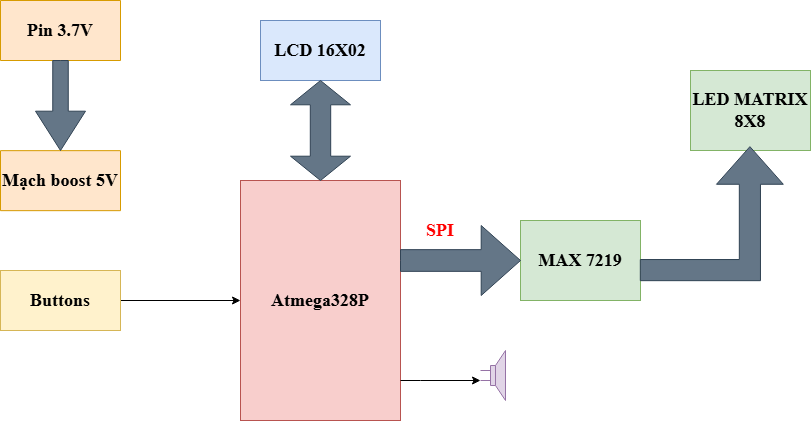
\includegraphics[width=.6\textwidth]{img/blockdiagram.png}
    \caption{Sơ đồ khối}
\end{figure}
\subsection{Sơ đồ nguyên lý (Schematics)}
\textbf{\textit{Khối vi xử lý trung tâm ATmega328P}}
\begin{figure}[h!]
    \centering
    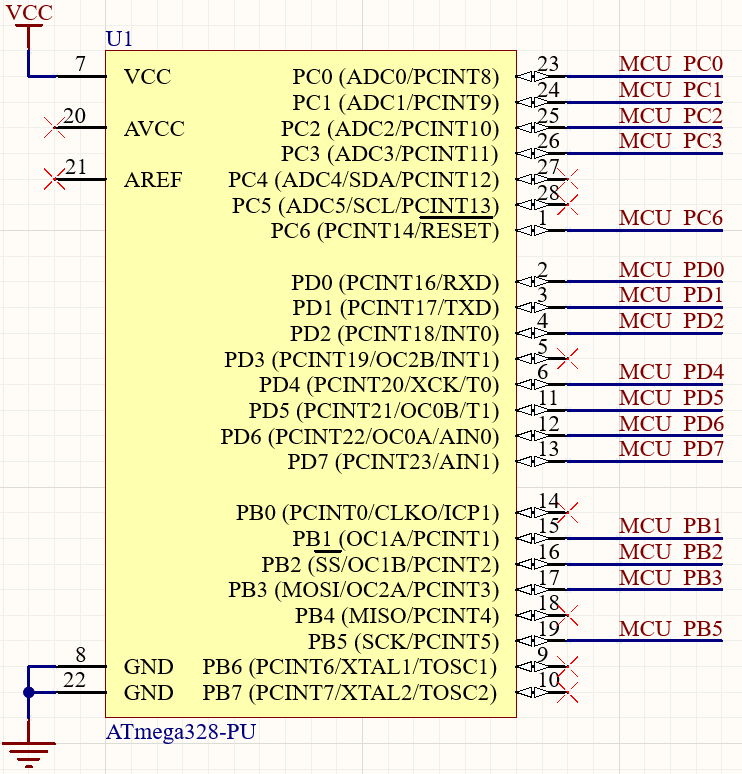
\includegraphics[width=.35\textwidth]{img/SCHEM_MCU.png}
    \caption{Khối vi xử lý trung tâm}
\end{figure}

\textbf{\textit{Khối giao tiếp LCD 1602}}
\begin{figure}[h!]
    \centering
    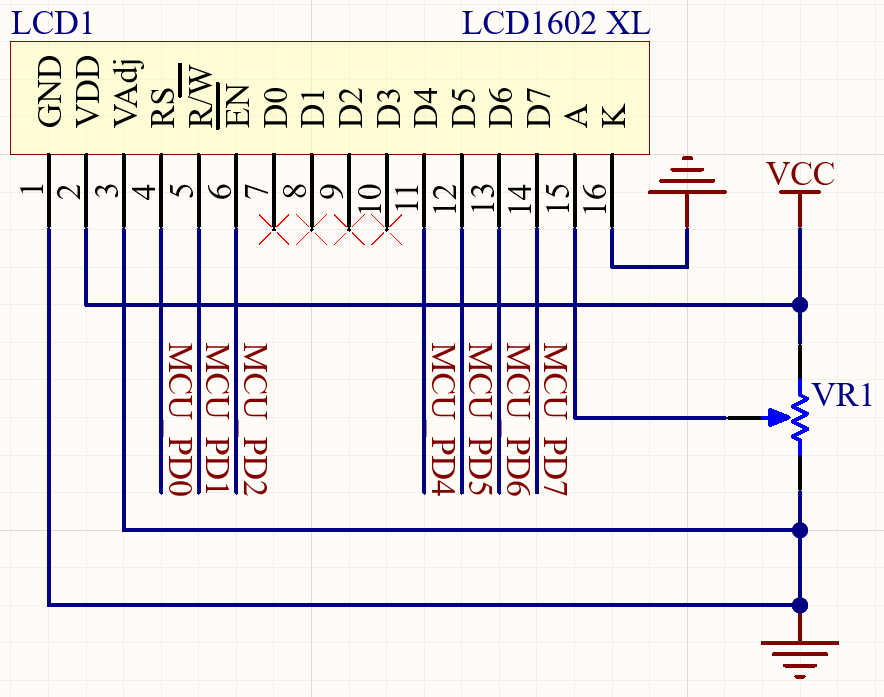
\includegraphics[width=.4\textwidth]{img/SCHEM_LCD.png}
    \caption{Khối giao tiếp LCD 1602}
\end{figure}

\textbf{\textit{Khối giao tiếp Buzzer}}
\begin{figure}[h!]
    \centering
    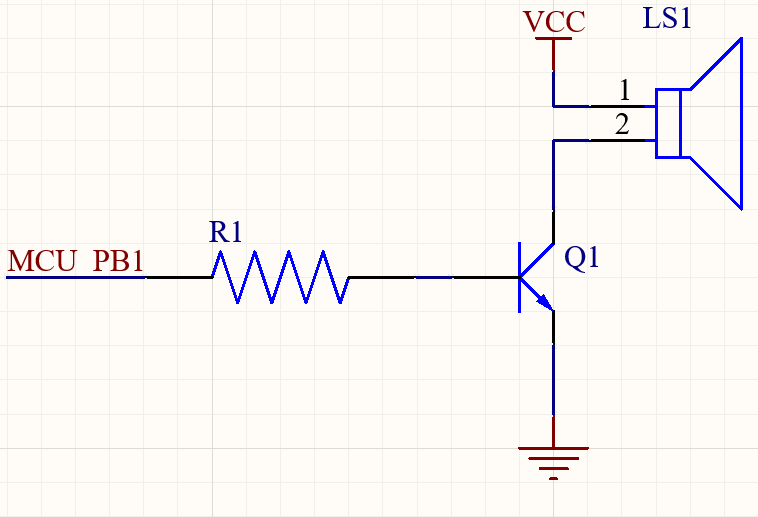
\includegraphics[width=.3\textwidth]{img/SCHEM_BUZZER.png}
    \caption{Khối giao tiếp Buzzer}
\end{figure}

\textbf{\textit{Khối giao tiếp Led ma trận}}
\begin{figure}[h!]
    \centering
    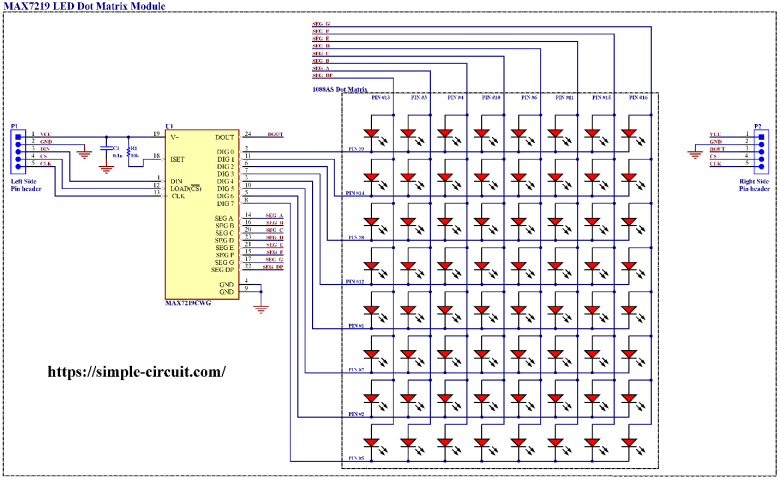
\includegraphics[width=.7\textwidth]{img/LED_MATRIX.png}
    \caption{Khối giao tiếp Led ma trận}
\end{figure}

\textbf{\textit{Khối giao tiếp nút nhấn}}
\begin{figure}[h!]
    \centering
    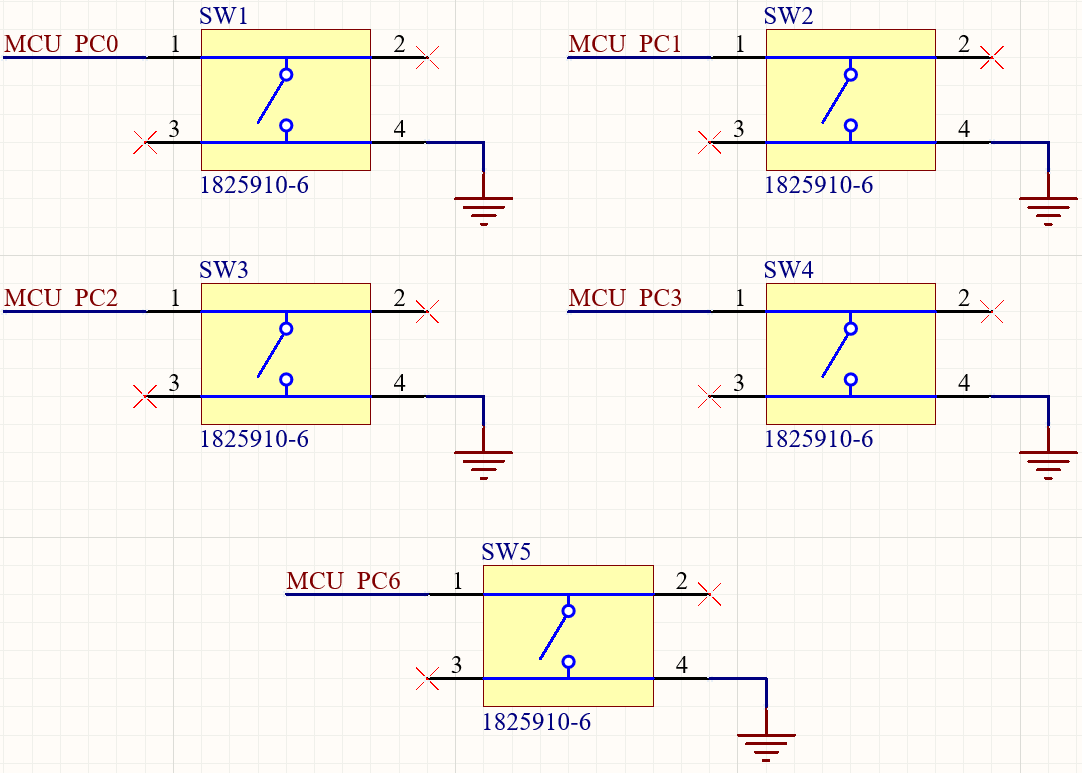
\includegraphics[width=.55\textwidth]{img/SCHEM_SW.png}
    \caption{Khối giao tiếp nút nhấn}
\end{figure}
\newpage
\textbf{\textit{Khối mạch sạc}}
\begin{figure}[h!]
    \centering
    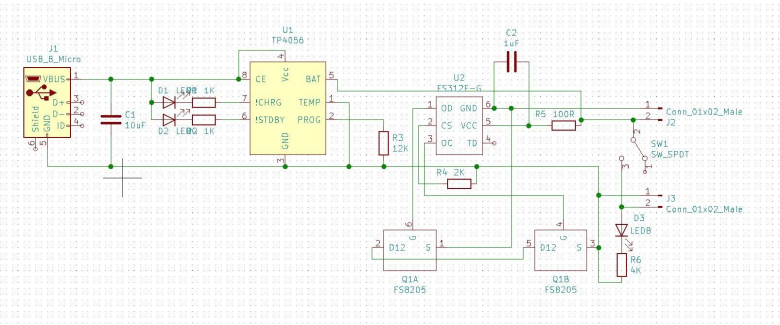
\includegraphics[width=.8\textwidth]{img/TP4056.png}
    \caption{Khối mạch sạc}
\end{figure}

\textbf{\textit{Khối mạch tăng áp}}
\begin{figure}[h!]
    \centering
    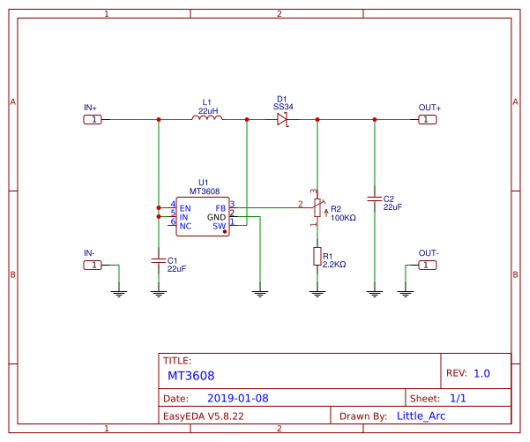
\includegraphics[width=.6\textwidth]{img/MT3608.png}
    \caption{Khối mạch tăng áp}
\end{figure}